\section{ストレッチセンサ計測アルゴリズム}
\ref{sec:RC回路}にて示す通り、ストレッチセンサの静電容量変化の計測にはRC回路を用いた時定数の計測で行った。
なお、この時定数の計測にはNucleoF303K8といったマイコン評価ボードを使用した。また、それらのコードの記述にはmbedライブラリを使用した。
使用したソースコードは下記リンクにて公開している。計測アルゴリズムはFig.\ref{fig:algorithm}にて示すように
1000Hzで計測を実行し、100Hzごとに計測データの平均値をSerial通信を用いてPCに出力した。
また、2000Hzで出力ピンの状態を切り替え、ストレッチセンサに電荷が残らないようにした。

ソースコード:https://os.mbed.com/users/HidetoN/code/Cap-Sensor/

\begin{figure}[h]
    \begin{center}
     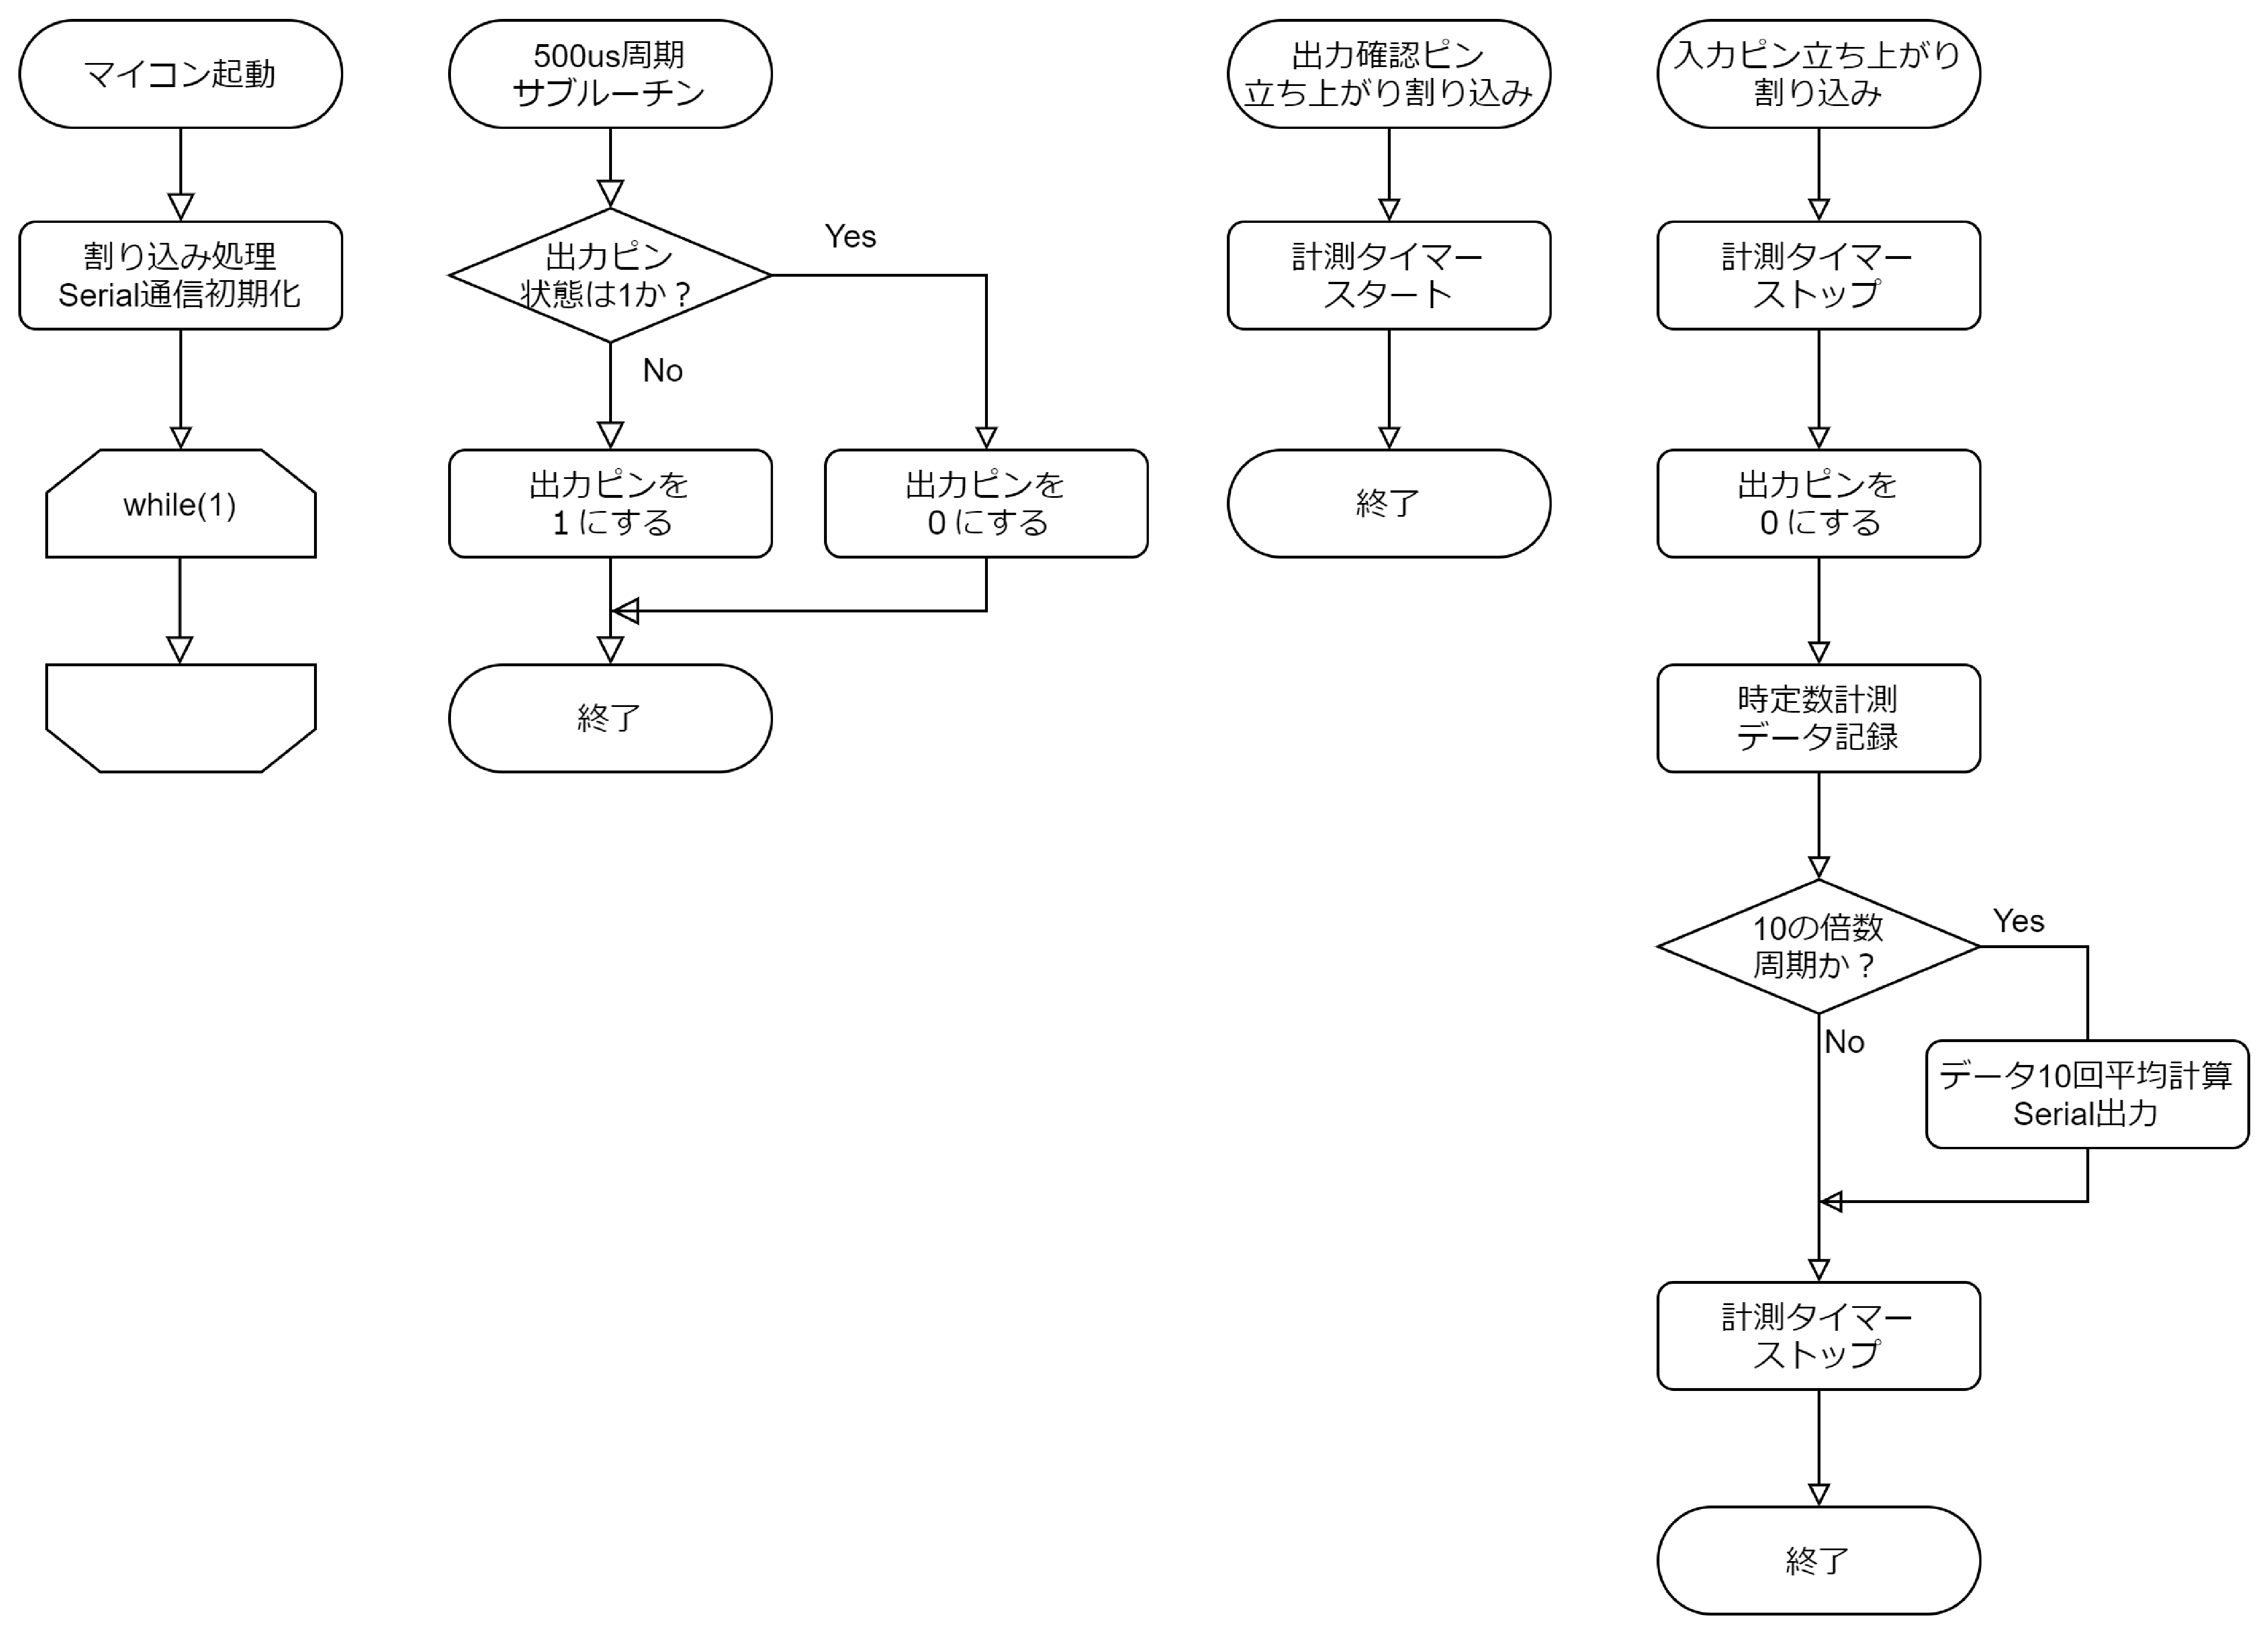
\includegraphics[width=0.9\columnwidth,clip]{./3_analysis/algorithm.eps}
     \caption{計測プログラムにおけるアルゴリズム}
     \label{fig:algorithm}
    \end{center}
\end{figure}

\section{足関節ロボット駆動システム}
足関節ロボットの駆動システムには従来から存在するペダリングロボット、2足歩行ロボットのシステムと同様のシステムを利用した。

Fig.\ref{fig:compressor}にて示した、エアーコンプレッサーで8気圧まで圧縮空気を作成し、気圧調整弁を用いて6気圧まで減圧を行った。

\begin{figure}[h]
    \begin{center}
     
\includegraphics[width=0.65\columnwidth,clip]{./3_analysis/compressor.eps}
     \caption{使用したエアーコンプレッサー}
     \label{fig:compressor}
    \end{center}
\end{figure}

\begin{figure}[h]
    \begin{center}
     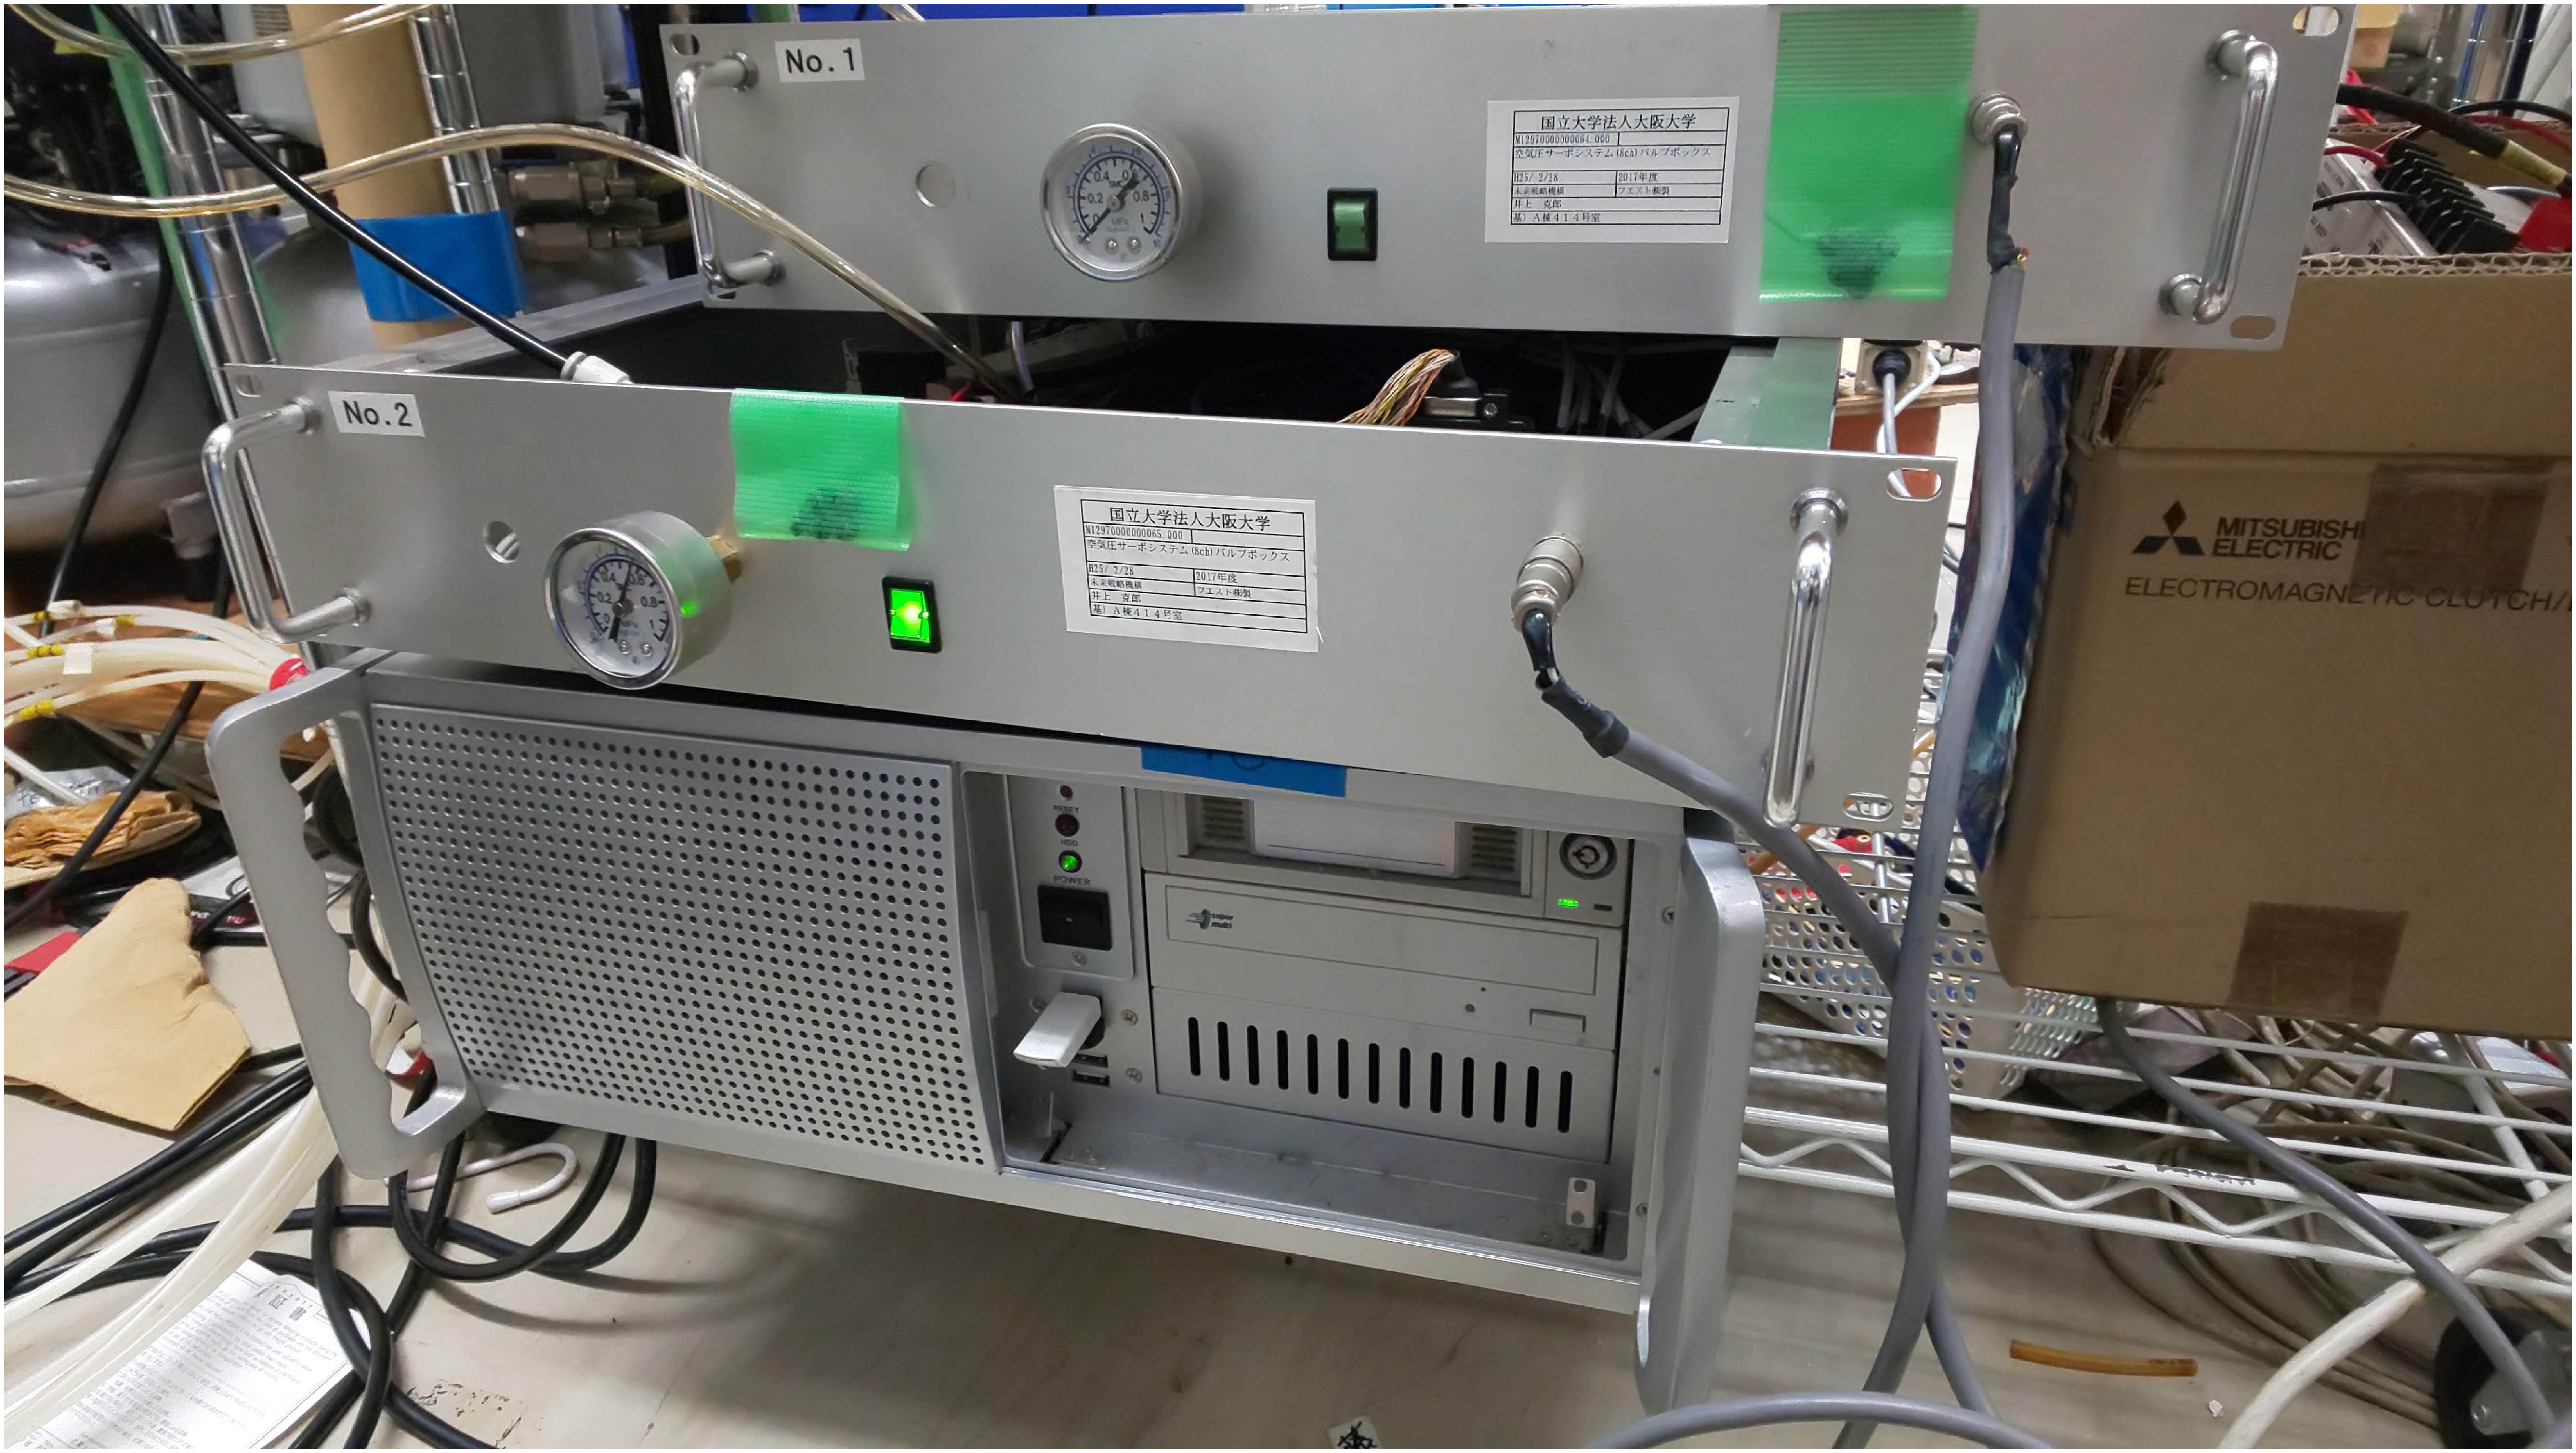
\includegraphics[width=0.65\columnwidth,clip]{./3_analysis/PC.eps}
     \caption{制御PCとエアー制御盤}
     \label{fig:PC}
    \end{center}
\end{figure}


Visual Studio 2010 C++ を用いたMFCアプリケーションを用いた

空気圧電磁弁への電圧指令(0~550)を記述したtxtファイル読み込み

AD変換ボード

\section{ストレッチセンサ計測データ処理}
